\graphicspath{{./images/}}

\chapter{Bausteinsicht}

\section{Beschreibung}

Die Architektur für die Applikation wird mittels vier Schichten realisiert. Die Präsentationsschicht ist auf dem WebServer während die anderen drei sich auf dem AppServer befinden. Die einzelnen Komponenten wurden gruppiert um die Übersicht zu wahren. Auf der nächsttieferen Ebene sind diese Komponenten detailierter aufgeführt.


\newgeometry{left=2.5cm, right=2.5cm, bottom=2.5cm, top=2.5cm}
\begin{landscape}
\section{Ebene 1}

\begin{center}
	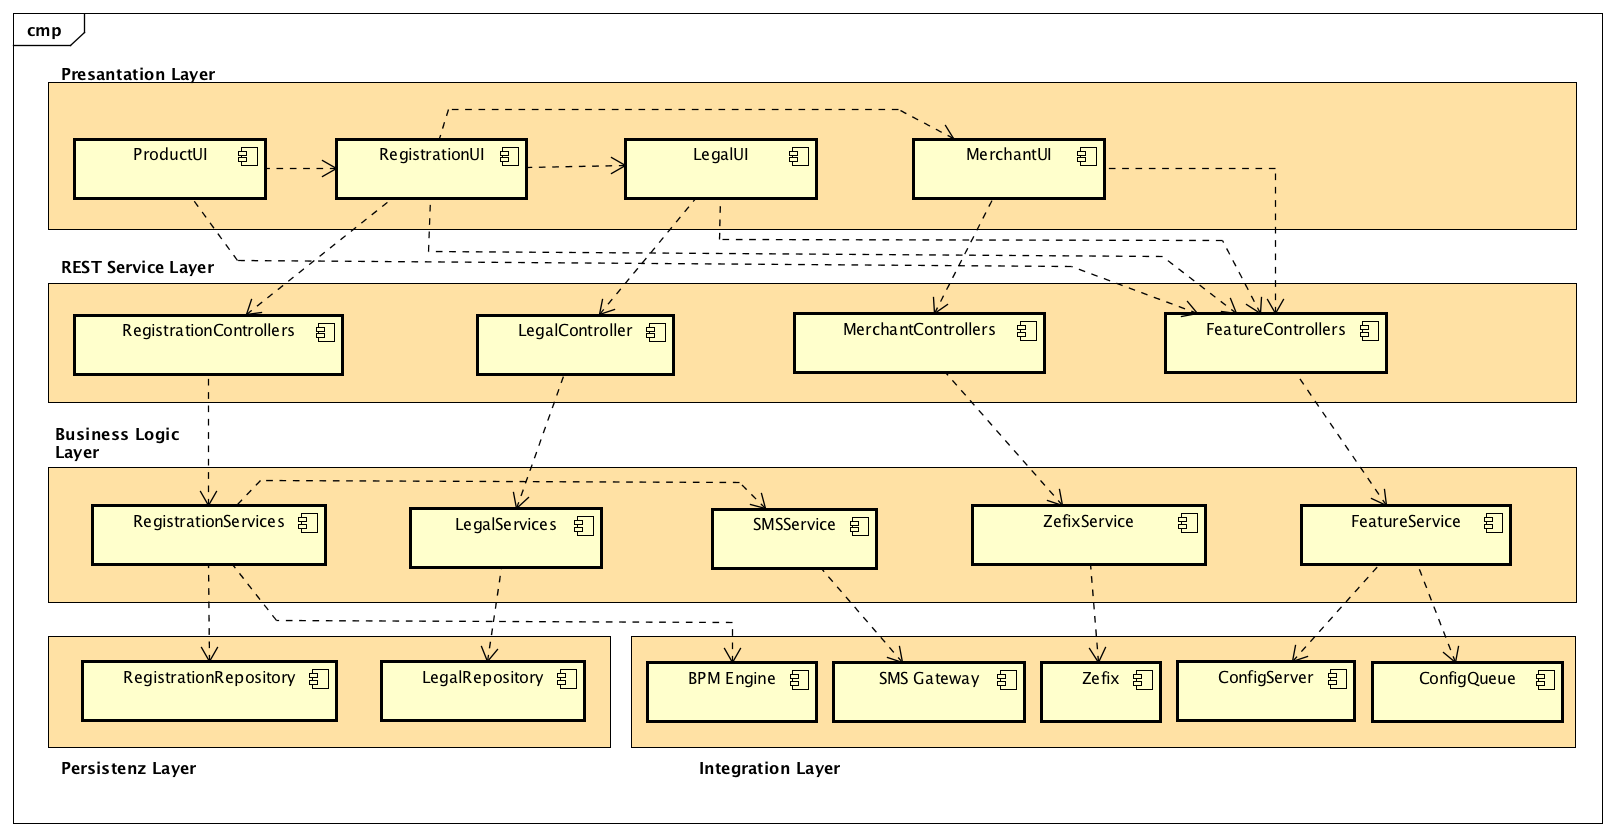
\includegraphics[scale=0.6]{ComponentLevel1.png}
\end{center}

\end{landscape}
\restoregeometry

\section{Ebene 2}

\section{Ebene 3}